\documentclass[10pt,a4paper]{beamer}
\usepackage[utf8]{inputenc}
\usepackage{amsmath}
\usepackage{amsfonts}
\usepackage{amssymb}
\usepackage{graphicx}
\author{Sunil T T }
 
 
\usepackage{listings}
\usepackage{color}
 
\definecolor{codegreen}{rgb}{0,0.6,0}
\definecolor{codegray}{rgb}{0.5,0.5,0.5}
\definecolor{codepurple}{rgb}{0.58,0,0.82}
\definecolor{backcolour}{rgb}{0.95,0.95,0.92}
 
\lstdefinestyle{mystyle}{
    backgroundcolor=\color{backcolour},   
    commentstyle=\color{codegreen},
    keywordstyle=\color{magenta},
    numberstyle=\tiny\color{codegray},
    stringstyle=\color{codepurple},
    basicstyle=\footnotesize,
    breakatwhitespace=false,         
    breaklines=true,                 
    captionpos=b,                    
    keepspaces=true,                 
    numbers=left,                    
    numbersep=5pt,                  
    showspaces=false,                
    showstringspaces=false,
    showtabs=false,                  
    tabsize=2
}
 
\lstset{style=mystyle}

 
 
\definecolor{links}{HTML}{2A1B81}
\hypersetup{colorlinks,linkcolor=,urlcolor=links}
%----------------------------------------------------------------------------------------
%	PACKAGES AND THEMES
%----------------------------------------------------------------------------------------


\mode<presentation> {

% The Beamer class comes with a number of default slide themes
% which change the colors and layouts of slides. Below this is a list
% of all the themes, uncomment each in turn to see what they look like.

%\usetheme{default}
%\usetheme{AnnArbor}
%\usetheme{Antibes}
%\usetheme{Bergen}
%\usetheme{Berkeley}
%\usetheme{Berlin}
%\usetheme{Boadilla}
\usetheme{CambridgeUS}
%\usetheme{Copenhagen}
%\usetheme{Darmstadt}
%\usetheme{Dresden}
%\usetheme{Frankfurt}
%\usetheme{Goettingen}
%\usetheme{Hannover}
%\usetheme{Ilmenau}
%\usetheme{JuanLesPins}
%\usetheme{Luebeck}
%\usetheme{Madrid}
%\usetheme{Malmoe}
%\usetheme{Marburg}
%\usetheme{Montpellier}
%\usetheme{PaloAlto}
%\usetheme{Pittsburgh}
%\usetheme{Rochester}
%\usetheme{Singapore}
%\usetheme{Szeged}
%\usetheme{Warsaw}

% As well as themes, the Beamer class has a number of color themes
% for any slide theme. Uncomment each of these in turn to see how it
% changes the colors of your current slide theme.

%\usecolortheme{albatross}
\usecolortheme{beaver}
%\usecolortheme{beetle}
%\usecolortheme{crane}
%\usecolortheme{dolphin}
%\usecolortheme{dove}
%\usecolortheme{fly}
%\usecolortheme{lily}
%\usecolortheme{orchid}
%\usecolortheme{rose}
%\usecolortheme{seagull}
%\usecolortheme{seahorse}
%\usecolortheme{whale}
%\usecolortheme{wolverine}

%\setbeamertemplate{footline} % To remove the footer line in all slides uncomment this line
%\setbeamertemplate{footline}[page number] % To replace the footer line in all slides with a simple slide count uncomment this line

%\setbeamertemplate{navigation symbols}{} % To remove the navigation symbols from the bottom of all slides uncomment this line
}

\usepackage{graphicx} % Allows including images
\usepackage{booktabs} % Allows the use of \toprule, \midrule and \bottomrule in tables
\usepackage{scrextend}
%----------------------------------------------------------------------------------------
%	TITLE PAGE
%----------------------------------------------------------------------------------------

\title[EC1302]{ Introduction to  git \\ \textcolor{blue}{ } } % The short title appears at the bottom of every slide, the full title is only on the title page

\author{Sunil Thomas T} % Your name
\institute[College of Engineering Attingal] % Your institution as it will appear on the bottom of every slide, may be shorthand to save space
{College of Engineering Attingal
\\ % Your institution for the title page
\medskip
\textit{suniltt@gmail.com} % Your email address
}
\date{\today} % Date, can be changed to a custom date

\begin{document}
 \begin{frame}
\titlepage % Print the title page as the first slide
\end{frame}


\begin{frame}
\frametitle{  Why you need version control}


\end{frame}

%------------------------------------------------

\begin{frame}[fragile]
\frametitle{  Installing git}
\begin{itemize}
    
    \item windows
    \item  linux
\end{itemize}

Initial configuration

\begin{lstlisting}[language=bash]

 git config --global user.name "Dr.Sunil"
 git config --global user.email "suniltt@gmail.com"
 
\end{lstlisting}
\end{frame}

%------------------------------------------------

\begin{frame}[fragile]
\frametitle{  Initialize git repository}

Create a new folder. Move to that folder.
\begin{lstlisting}[language=bash]
 git init
 
\end{lstlisting}
\pause

What happens when you do git init.  

A hidden folder containing the repository is created. Examine that folder. ( Control h for viewing hidden files)

 \begin{figure}
  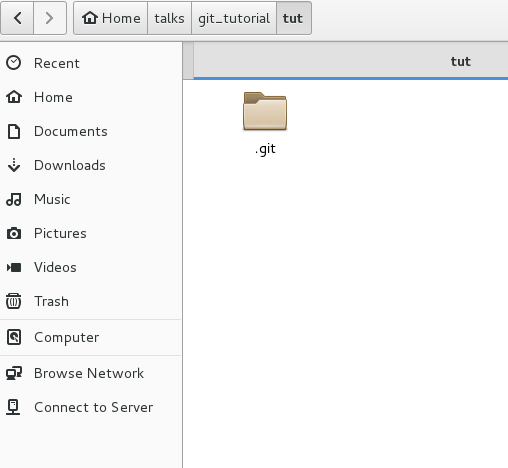
\includegraphics[scale=.4]{2}
 \end{figure}
 
  \begin{figure}
  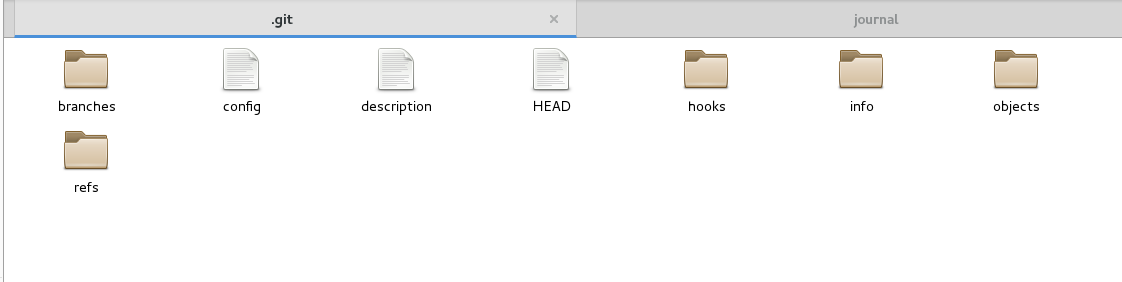
\includegraphics[scale=.4]{3}
 \end{figure}
\end{frame}



\begin{frame}[fragile]
\frametitle{  Inside the git repo}
  \begin{figure}
  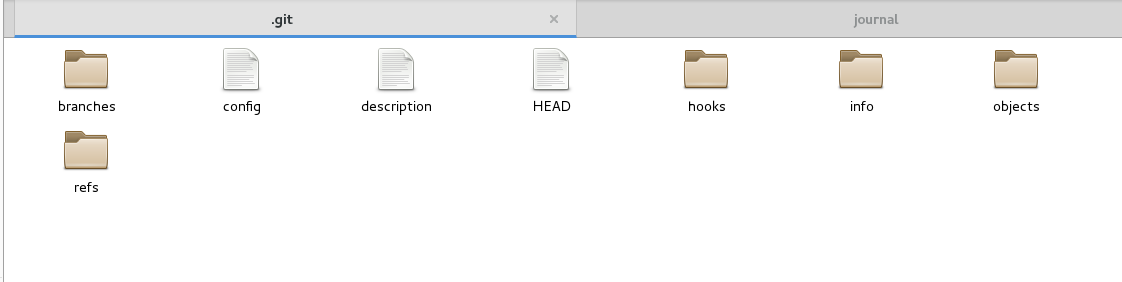
\includegraphics[scale=.35]{3}
 \end{figure}

\end{frame}




\begin{frame}[fragile]
\frametitle{ Git work flow}

  \begin{figure}
  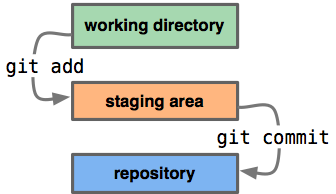
\includegraphics[scale=.6]{1}
 \end{figure}


\end{frame}

\begin{frame}[fragile]
\frametitle{  Examine git status}

\begin{lstlisting}[language=bash]
 git status
 
\end{lstlisting}


  \begin{figure}
  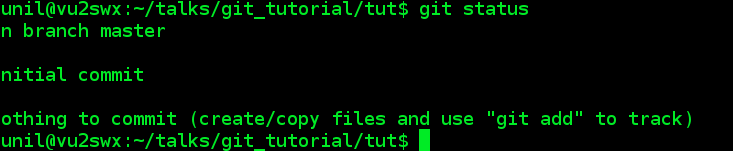
\includegraphics[scale=.4]{4}
 \end{figure}


\end{frame}

\begin{frame}[fragile]
\frametitle{  }
Add a file to your working directory.
  \begin{figure}
  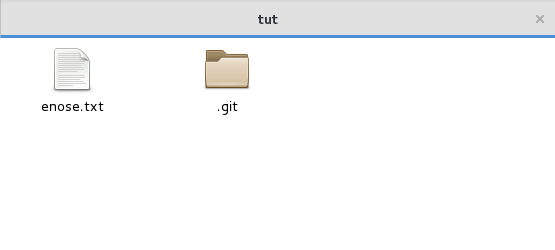
\includegraphics[scale=.4]{5}
 \end{figure}
 
 
 \begin{lstlisting}[language=bash]
 git status
 
\end{lstlisting}
 \begin{figure}
  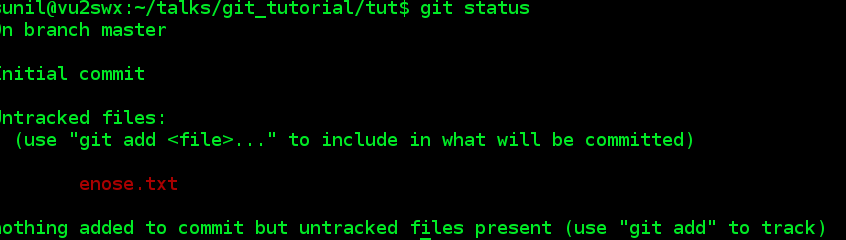
\includegraphics[scale=.4]{6}
 \end{figure}

\end{frame}

\begin{frame}[fragile]
\frametitle{  Add the file to staging area }
 \begin{lstlisting}[language=bash]
 git  add enose.txt
 git status 
\end{lstlisting}
\begin{figure}
  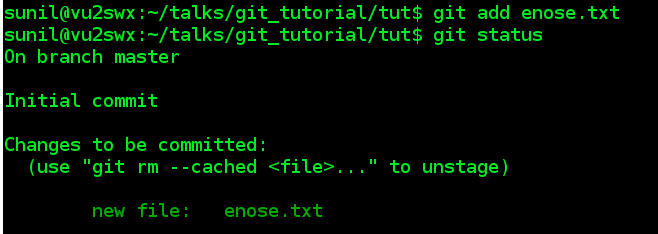
\includegraphics[scale=.4]{7}
 \end{figure}
\end{frame}

\begin{frame}[fragile]
\frametitle{ Commit changes }
 \begin{lstlisting}[language=bash]
 git  commit -m "initial commit"  enose.txt
 
\end{lstlisting}
\begin{figure}
  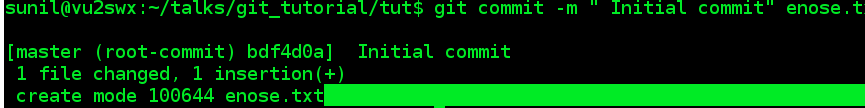
\includegraphics[scale=.4]{8}
 \end{figure}
 

\end{frame}

\begin{frame}[fragile]
\frametitle{  Add more files}

\begin{figure}
  
\includegraphics[scale=.4]{9}
 \end{figure}

  \begin{lstlisting}[language=bash]
 git  add enose.bib
 git status 
 git commit -m " Added bibliography" enose.bib
\end{lstlisting}

\end{frame}


\begin{frame}
\frametitle{  Still more files }
\begin{figure}
  
\includegraphics[scale=.4]{10}
 \end{figure}
 
% 
%  \begin{lstlisting}[language=bash]
% git  add drawing.fig
% git status 
% git commit -m " Added fig" drawing.fig
%\end{lstlisting}
\end{frame}




\begin{frame}[fragile]
\frametitle{  Commit more files}

 
  \begin{lstlisting}[language=bash]
 git  add drawing,fig
 git status 
 git commit -m " Added drawing" drawing,fig
\end{lstlisting}

\end{frame}



\begin{frame}[fragile]
\frametitle{  Let us see the history }
 \begin{lstlisting}[language=bash]
 git  log
\end{lstlisting}
\begin{figure}
  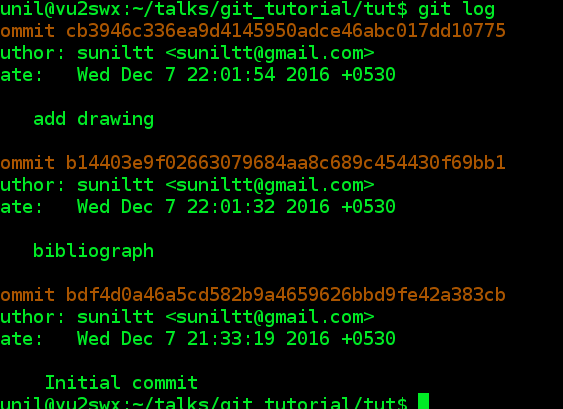
\includegraphics[scale=.4]{11}
 \end{figure}
\end{frame}






 

\begin{frame}[fragile]
\frametitle{  Checkout}

 Now let us edit enose  txt. After some editing we see that we want to restore the saved copy.
  \begin{lstlisting}[language=bash]
 git status
 git  checkout enose.txt
 git status
\end{lstlisting}

\end{frame}

\begin{frame}[fragile]
\frametitle{  Checkout from previous commits}
 
 Get the commit commit id
  \begin{lstlisting}[language=bash]
  git log --oneline

\end{lstlisting}

\begin{figure}
  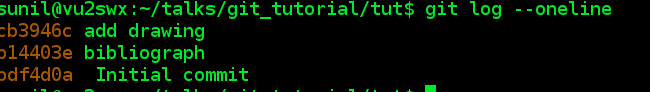
\includegraphics[scale=.4]{12}
 \end{figure}
 
You can check out from any previous commits using the commit id
\begin{figure}
  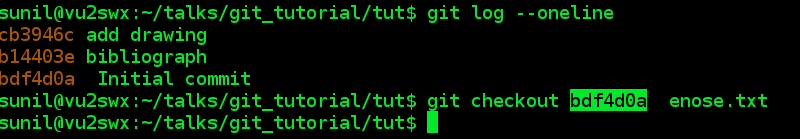
\includegraphics[scale=.4]{13}
 \end{figure}
  
\end{frame}

\begin{frame}[fragile]
\frametitle{  Creating a new branch}

  
  \begin{lstlisting}[language=bash]
 git status
 git  branch ieee
 git checkout ieee
 git status
\end{lstlisting}

Do your editing on branch ieee. You can add files. commit and do all sort of operations.
Now we want to switch back to master branch.

  \begin{lstlisting}[language=bash]
 git status
 
 git checkout master
 git status
\end{lstlisting}
\end{frame}




\begin{frame}[fragile]
\frametitle{  }

  Check out ieee branch and add few more files to your ieee baranch and commit
  \begin{lstlisting}[language=bash]
 git status
 git  checkout ieee
 git status
\end{lstlisting}

\begin{figure}
  
\includegraphics[scale=.3]{15}
 \end{figure}

\begin{figure}
  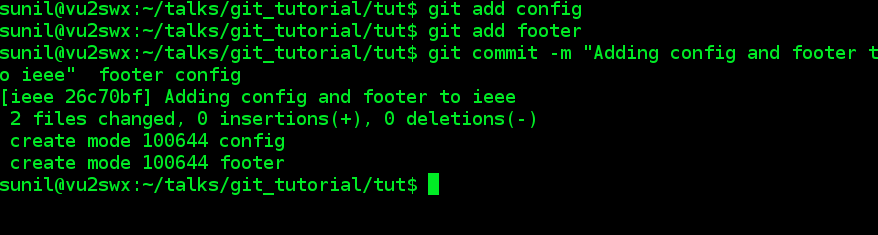
\includegraphics[scale=.3]{16}
 \end{figure}

\end{frame}



\begin{frame}[fragile]
\frametitle{  }

  Check out master branch 
  \begin{lstlisting}[language=bash]
 git status
 git  checkout master
 git status
\end{lstlisting}

See the files from ieee branch vanish.
\begin{figure}
  
\includegraphics[scale=.3]{17}
 \end{figure}
 
\end{frame}


\begin{frame}[fragile]
\frametitle{ Merge branches  }

  Check out master branch 
  \begin{lstlisting}[language=bash]
 git status
 git  checkout master
 git status
 git merge ieee
\end{lstlisting}

 
\begin{figure}
  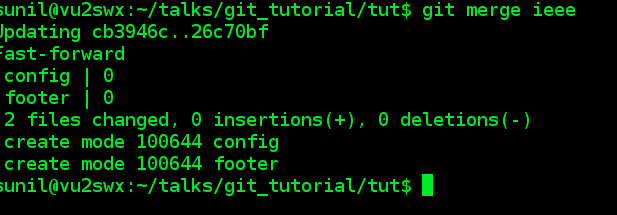
\includegraphics[scale=.3]{18}
 \end{figure}
 
 Delete a branch 
   \begin{lstlisting}[language=bash]
 git status
 
 
 git branch  -d ieee
\end{lstlisting}
\end{frame}


\begin{frame}[fragile]
\frametitle{ Reverting Merge  }

  
 
\begin{figure}
  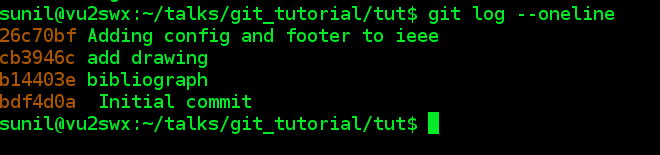
\includegraphics[scale=.3]{19}
 \end{figure}
  
  
  \begin{figure}
  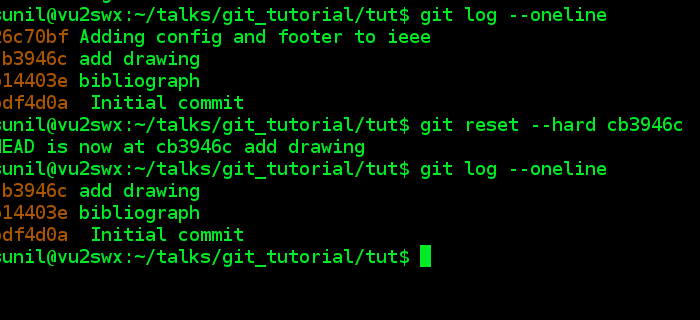
\includegraphics[scale=.3]{20}
 \end{figure}
\end{frame}



\begin{frame}[fragile]
\frametitle{ Viewing an older version }

  
 
\begin{figure}
  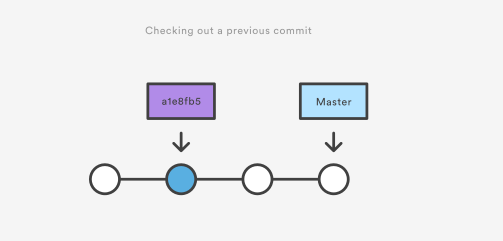
\includegraphics[scale=.3]{21}
 \end{figure}
  
  Get commit id 
  \begin{lstlisting}[language=bash]
 git log --online
 
\end{lstlisting}

Checkout 
    \begin{lstlisting}[language=bash]
 git checkout b14403e
 
\end{lstlisting}

To get back the master version
   \begin{lstlisting}[language=bash]
 git checkout master
 
\end{lstlisting}

\end{frame}
 
\begin{frame}[fragile]
\frametitle{ reverting to older version }

\begin{figure}
  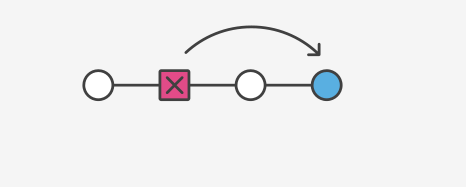
\includegraphics[scale=.3]{22}
 \end{figure}
  
  Get commit id 
  \begin{lstlisting}[language=bash]
 git  revert <commit id>
 
\end{lstlisting}


\end{frame}


 
\begin{frame}[fragile]
\frametitle{ Collaborating }

 Go to git hub. Create an account. Verify.  Create a repository under your login.

\end{frame}


 
\begin{frame}[fragile]
\frametitle{ Collaborating }
 
\begin{figure}
  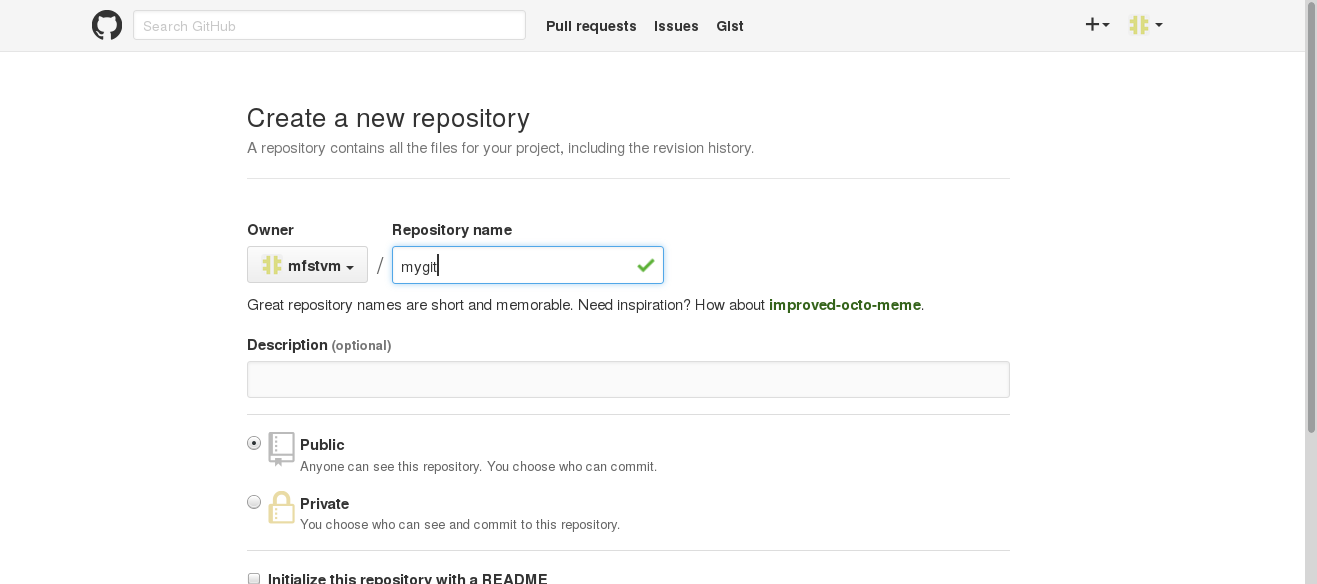
\includegraphics[scale=.3]{24}
 \end{figure}
\end{frame}

\begin{frame}[fragile]
\frametitle{ Collaborating }
 
\begin{figure}
  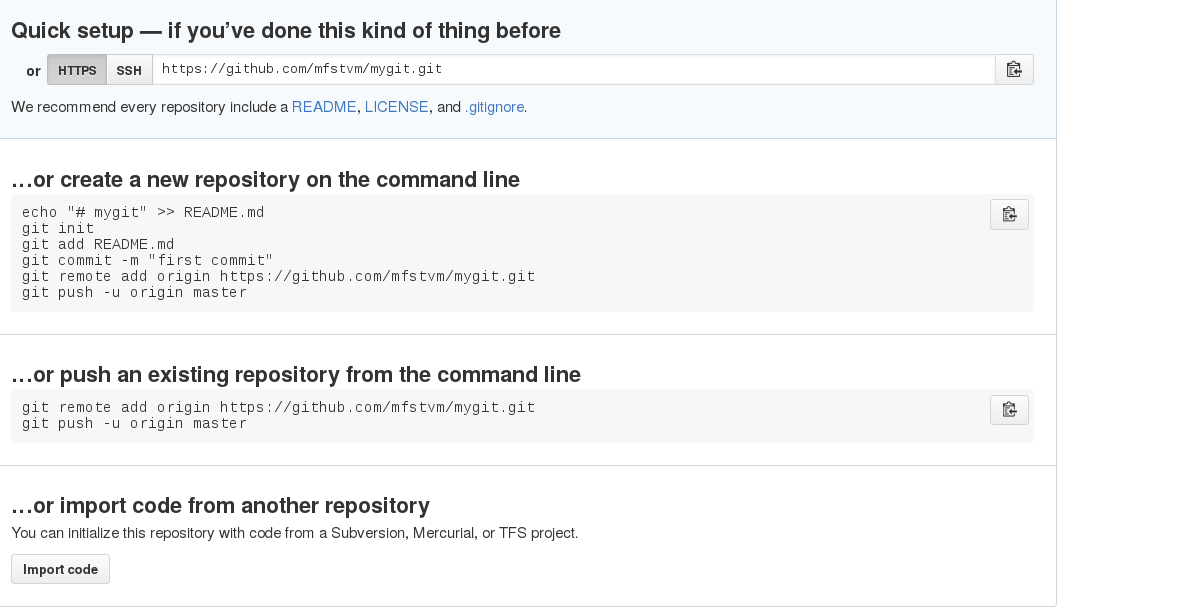
\includegraphics[scale=.3]{25}
 \end{figure}
\end{frame}
%
% 
%
%\begin{frame}
%\frametitle{  Why you need version control}
%
%
%\end{frame}
%
%\begin{frame}
%\frametitle{  Why you need version control}
%
%
%\end{frame}
%
%\begin{frame}
%\frametitle{  Why you need version control}
%
%
%\end{frame}
%
%\begin{frame}
%\frametitle{  Why you need version control}
%
%
%\end{frame}
%
%
%

\end{document} 

